% !TeX program = pdfLaTeX
\documentclass[smallextended]{svjour3}       % onecolumn (second format)
%\documentclass[twocolumn]{svjour3}          % twocolumn
%
\smartqed  % flush right qed marks, e.g. at end of proof
%
\usepackage{amsmath}
\usepackage{graphicx}
\usepackage[utf8]{inputenc}

\usepackage[hyphens]{url} % not crucial - just used below for the URL
\usepackage{hyperref}
\providecommand{\tightlist}{%
  \setlength{\itemsep}{0pt}\setlength{\parskip}{0pt}}

%
% \usepackage{mathptmx}      % use Times fonts if available on your TeX system
%
% insert here the call for the packages your document requires
%\usepackage{latexsym}
% etc.
%
% please place your own definitions here and don't use \def but
% \newcommand{}{}
%
% Insert the name of "your journal" with
% \journalname{myjournal}
%

%% load any required packages here



\newlength{\cslhangindent}
\setlength{\cslhangindent}{1.5em}
\newenvironment{cslreferences}%
  {\setlength{\parindent}{0pt}%
  \everypar{\setlength{\hangindent}{\cslhangindent}}\ignorespaces}%
  {\par}

\usepackage{kotex}
\usepackage{booktabs}
\usepackage{longtable}
\usepackage{array}
\usepackage{multirow}
\usepackage{wrapfig}
\usepackage{float}
\usepackage{colortbl}
\usepackage{pdflscape}
\usepackage{tabu}
\usepackage{threeparttable}
\usepackage{threeparttablex}
\usepackage[normalem]{ulem}
\usepackage{makecell}
\usepackage{xcolor}

\begin{document}

\title{자동화에 따른 노동시간 변화 분석 }



\author{  이광춘 \and  주용우 \and  }


\institute{
        이광춘 \at
     연세대학교 상경대학 응용통계학과 \\
     \email{\href{mailto:kwangchun.lee.7@gmail.com}{\nolinkurl{kwangchun.lee.7@gmail.com}}}  %  \\
%             \emph{Present address:} of F. Author  %  if needed
    \and
        주용우 \at
     연세대학교 상경대학 응용통계학과 \\
     \email{\href{mailto:yongwoo96@yonsei.ac.kr}{\nolinkurl{yongwoo96@yonsei.ac.kr}}}  %  \\
%             \emph{Present address:} of F. Author  %  if needed
    \and
    }

\date{Received: date / Accepted: date}
% The correct dates will be entered by the editor


\maketitle

\begin{abstract}
알파고가 2016년 바둑 인간 챔피언 이세돌 9단을 현격한 기량차이로
격파하면서 인공지능에 대한 관심이 급격히 증가하였다. 그와 동시에
인공지능이 인간의 일자리를 대체하면서 막연한 불안감이 삽시간에
전파되었다. 기계와의 일자리 경쟁은 컴퓨터의 출현이전부터 시작되었지만
인간만의 고유한 영역으로 알고 있던 인지, 창작 등 다양한 분야에서 오히려
인간보다 더 우수한 성능을 보여주면서 인간의 일자리가 기계에 대체되는
것은 가시권에 들어섰다. 이번 문헌조사와 실증 데이터 분석을 통해서 기계가
인간의 일자리를 대체하는 자동화의 본질에 대해서 살펴보고, 인간과 기계의
업무 분장을 통해 더 생산성을 높일 수 있는 방안을 제시하고자 한다.
\\
\keywords{
        자동화 \and
        데이터 과학 \and
        인공지능 \and
        일자리 \and
        기계와 사람의 업무분장 \and
    }


\end{abstract}


\def\spacingset#1{\renewcommand{\baselinestretch}%
{#1}\small\normalsize} \spacingset{1}


\hypertarget{intro}{%
\section{들어가며}\label{intro}}

과거 숫자를 다룰 수 있는 소수의 사람만이 숫자의 계산을 암산에서 벗어나
주판의 도움으로 생산성을 주판을 사용하지 못한 사람과 비교하여 수십배에서
수천배의 정확도와 함께 빠른 계산을 달성하게 되었다. 이러한 주판은 중간에
기계장치 계산기(찰스 배비지)도 있었지만, 일제 전자계산기로 자리를
내어주지만 사칙연산만 이해하면 기존 주판과 비교하여 어마어마한 생산성을
향상과 정확도를 높인 것은 분명하다.

이후, 개인용 컴퓨터의 보급으로 비지칼크와 로터스 1-2-3가 그 가능성을
열었다면 마이크로소프트 엑셀 스프레드쉬트 프로그램이 세무사 업무의
생산성을 또한 엄창나게 올린 것도 사실이다.

이제 문제가 되는 것은
\href{https://www.pcmag.com/roundup/167894/the-best-tax-software}{PC
매거진, ``The Best Tax Software for 2019''}에 소개된 세금관련 프로그램이
\$39 달러에 불과하다는 점이다. 1년 세무업무가 개인의 경우 4만원에
불과한데 세무사가 이런 자동화된 기계와 경쟁에서 승리할 수 있는가? 결과는
명확하다.

그렇다면 세무사와 유사한 직업군으로 회계사를 들 수 있는데, 최근
인공지능의 발전은 단순히 숫자에만 머무르지 않고, 자연어 처리(NLP,
Natural Language Processing) 기술의 발전에 힘입어 기사를 써주는 로봇을
비롯하여 문자를 주로 다루는 대표적인 직업군인 법률/변호사 일자리도
위협하고 있다. 물론 이미지를 인식하는 인공지능 기술도 급격히 향상되어
의사를 비롯한 시각 인지 기술이 직업에 중요한 역할을 수행하는 직업군에도
향후 상당한 변화를 줄 것으로 예상된다.

\begin{figure}

{\centering 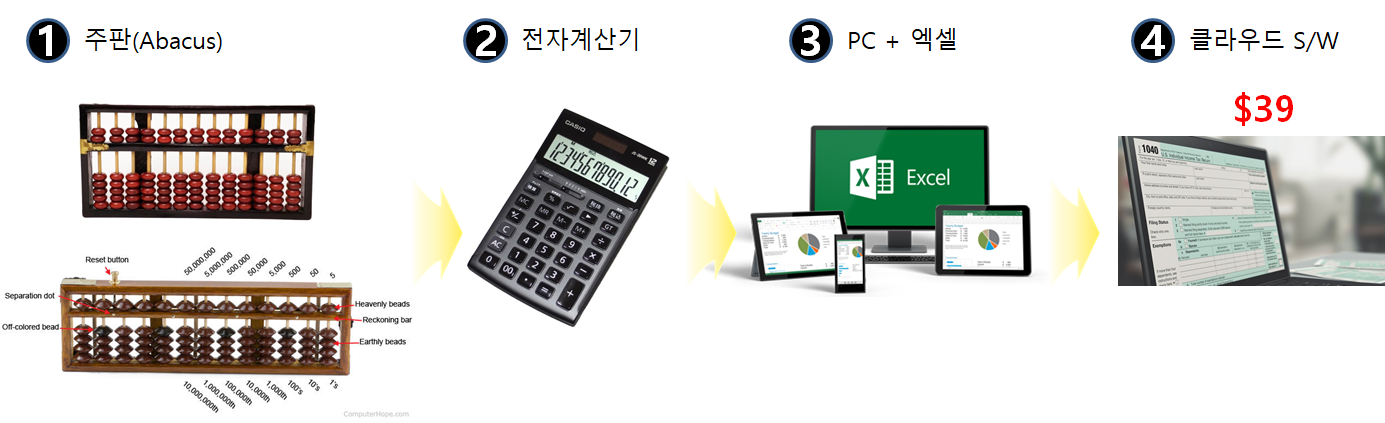
\includegraphics[width=1\linewidth]{fig/tax-preparation} 

}

\caption{세무 업무 변천사}\label{fig:unnamed-chunk-1}
\end{figure}

\hypertarget{sec:1}{%
\section[세무업무 자동화]{\texorpdfstring{세무업무
자동화\footnote{\href{https://www.pcmag.com/roundup/167894/the-best-tax-software}{PC
  매거진, ``The Best Tax Software for 2019''}}}{세무업무 자동화}}\label{sec:1}}

\href{http://biz.newdaily.co.kr/site/data/html/2019/01/22/2019012200053.html}{등록세무사만
1만3000명인데 합격자를 늘리다니\ldots{} 세무사회 불만 고조} 기사
내용에도 언급되었어듯이 2008년부터 11년간 630명가량을 다소 편차가 있지만
뽑아왔다. 현재 한국세무사회에 등록된
\href{http://www.kacpta.or.kr/}{개인 및 법인현황}을 통해 12,973명이
개업하여 활동하고 있는 것으로 집계되어 있다.

\begin{tabular}{ll}
\toprule
연도 & 합격자\\
\midrule
2012 & 654\\
2013 & 631\\
2014 & 631\\
2015 & 630\\
2016 & 634\\
\addlinespace
2017 & 630\\
2018 & \\
\bottomrule
\end{tabular}

\href{http://news.bizwatch.co.kr/article/tax/2018/10/05/0010}{임명규
(2018.10.10), ``세무사는 얼마나 벌까요'', Business Watch} 조사를 통해서
세무사 1인당 매출과 연봉 추정을 살펴볼 수 있다.

\hypertarget{automation-job-statistics}{%
\section{자동화와 직업 통계자료}\label{automation-job-statistics}}

급격한 자동화를 통한 직업변화를 하나의 요인만으로 살펴볼 수는 없다.
대표적으로 그동안 세계화 전략을 통한 제조와 생산에 필요한 인력을
인건비가 저렴한 해외에서 찾았으나 인공지능의 발전에 따라 글로벌
생산거점을 두고 생산하던 것보다 훨씬 경쟁력있게 됨에 따라 일자리에도
커다란 변화의 조짐이 일어나고 있다.

\hypertarget{strategy-change}{%
\subsection{소싱전략의 변화}\label{strategy-change}}

Kinetics consulting services / Automation Anywhere 자료에 의하면
비정규직 인력아웃소싱 비용도 현재 시점에서 사무 로봇을 사용하게 되면
더욱 줄일 수 있다는 조사결과를 제시하고 있다.

\begin{figure}

{\centering 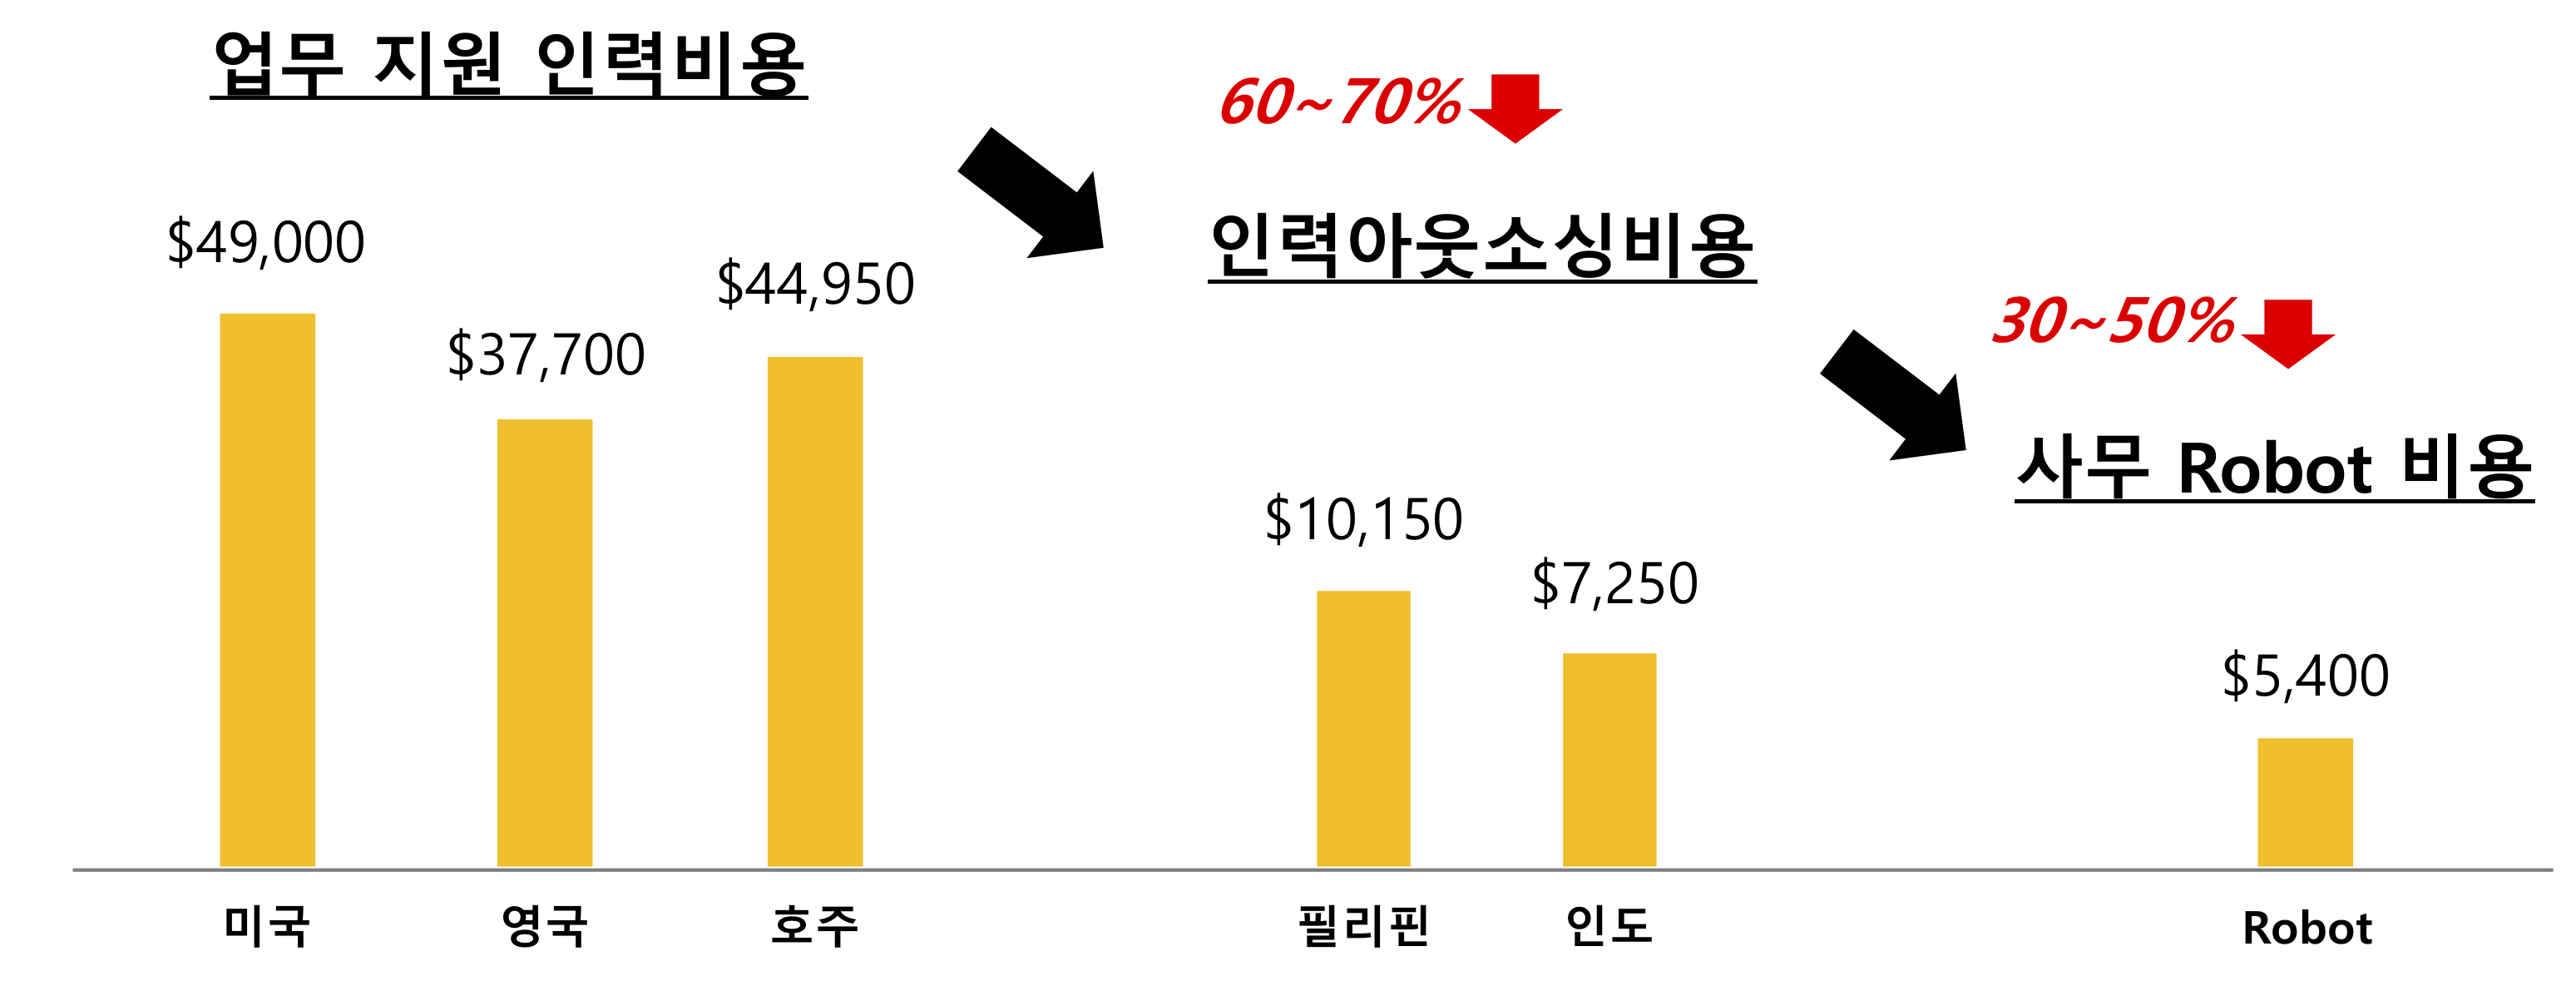
\includegraphics[width=1\linewidth]{fig/the-end-of-outsourcing} 

}

\caption{소싱 전략의 변화}\label{fig:unnamed-chunk-2}
\end{figure}

\hypertarget{industrial-robot}{%
\subsection[산업용 로봇]{\texorpdfstring{산업용
로봇\footnote{\href{https://www.visualcapitalist.com/industrial-robot-sales-sky-high/}{Ang
  Ahlstrom (May 24, 2018), ``Chart: Why Industrial Robot Sales are Sky
  High''}}}{산업용 로봇}}\label{industrial-robot}}

\href{https://www.visualcapitalist.com/industrial-robot-sales-sky-high/}{Ang
Ahlstrom (May 24, 2018), ``Chart: Why Industrial Robot Sales are Sky
High''} 기사에 언급되었듯이 2010년을 기점으로 산업용 로봇은 엄청난
성장세를 타고 있다. 특히, 2008년 금융위기를 기점으로 산업용 로봇 공급은
급격히 늘어나고 있다. 기사가 반영하지 못한 가장 최근 추세를 추가해서
시각화해 보면 그 범위와 자동화를 통한 일자리 영향이 어느 정도될지 예측이
가능하다.

\begin{center}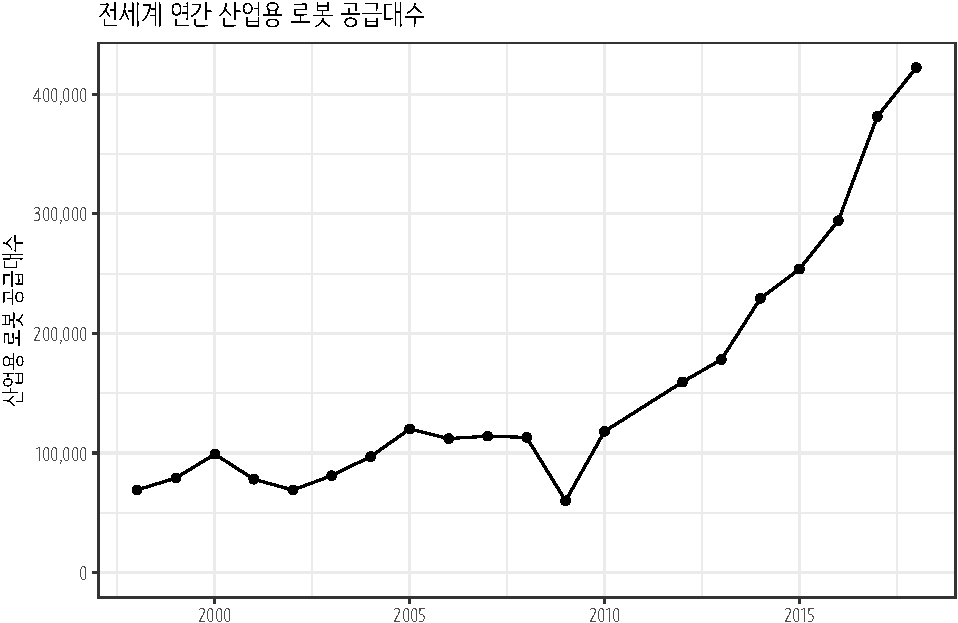
\includegraphics{paper_files/figure-latex/industrial-robot-1} \end{center}

\hypertarget{wage-productivity-gap}{%
\subsection{생산성과 임금 격차}\label{wage-productivity-gap}}

\href{https://www.epi.org/productivity-pay-gap/}{Economic Policy
Institute, ``The Productivity - Pay Gap'', July 2019}

생산성이 오르면 임금도 따라 오른 다는 것이 그동안의 믿음이었다. 하지만,
생산성이 오른다고 임금도 따라 오르지 않는 현상이 1979년부터 심화되고
있다. 이를 데이터를 통해서 확인해보자.

데이터 출처: EPI analysis of unpublished Total Economy Productivity data
from Bureau of Labor Statistics (BLS) Labor Productivity and Costs
program, wage data from the BLS Current Employment Statistics, BLS
Employment Cost Trends, BLS Consumer Price Index, and Bureau of Economic
Analysis National Income and Product Accounts Updated from Figure A in
Raising America's Pay: Why It's Our Central Economic Policy Challenge
(Bivens et al.~2014)

\begin{center}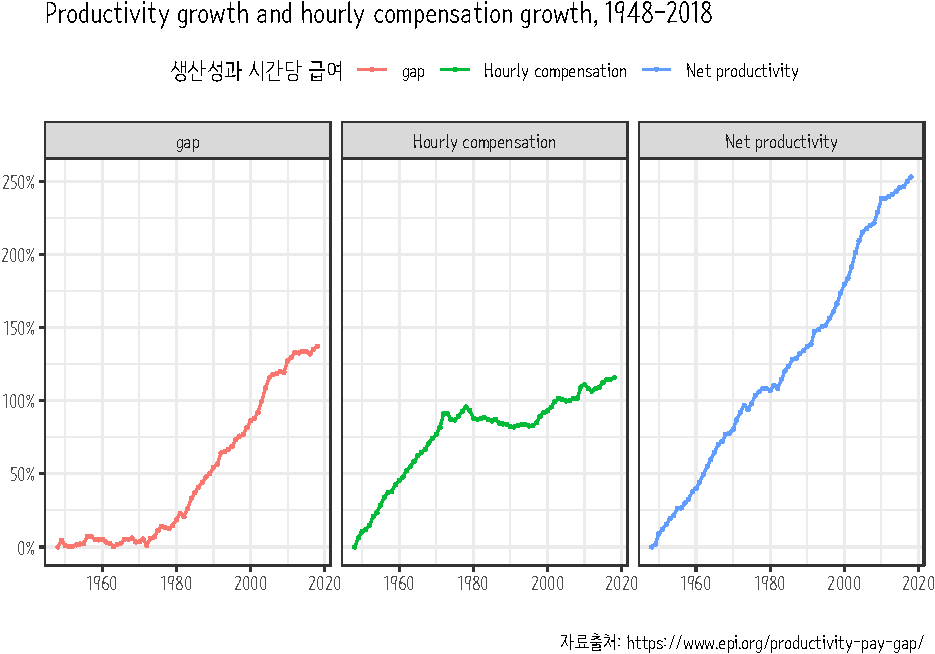
\includegraphics{paper_files/figure-latex/productivity-gap-1} \end{center}

\hypertarget{bowley-law}{%
\subsection{보울리 법칙(Bowley's Law)}\label{bowley-law}}

앞서 언급한 임금과 노동생산성 간 격차의 지속적 증가는 노동소득분배율
(labour income share)의 감소로 연결되는데, 노동소득분배율은 총국민소득
중 노동소득이 차지하는 비중으로 보울리의 법칙으로 불리며 경제성장이나
발전과는 상관없이 기능적 소득분배((functional income distribution))가
장기적으로 일정하다는 가설인데 이것이 최근 깨지고 있다.\footnote{\href{https://slownews.kr/24431}{이상혁(2014),
  ``제네바에서 온 편지: 당신의 월급은 공정합니까?'', slow news}}

FRED Economic Data 중
\href{https://fred.stlouisfed.org/series/W270RE1A156NBEA}{Shares of
gross domestic income: Compensation of employees, paid: Wage and salary
accruals: Disbursements: to persons (W270RE1A156NBEA)} 다운로드 받아
시각화한다. 미국 노동소득분배율이 50\%대에서 40\%초반으로 훅 떨어진 것이
시각적으로 확인된다. 이에 대해서 ILO 세계임금보고서와 다른
\href{https://www.oecd.org/g20/topics/employment-and-social-policy/The-Labour-Share-in-G20-Economies.pdf}{OECD
(2015), ``The Labour Share in G20 Economies''} 내용을 통해 다양한 원인을
살펴볼 수 있다.

\begin{itemize}
\tightlist
\item
  노동분배몫 하락 요인 (ILO 세계임금보고서, 2012)

  \begin{itemize}
  \tightlist
  \item
    산업구조 변화와 기술 변화
  \item
    세계화
  \item
    금융화(financialization)
  \item
    노동시장과 복지정책의 약화
  \end{itemize}
\end{itemize}

\begin{center}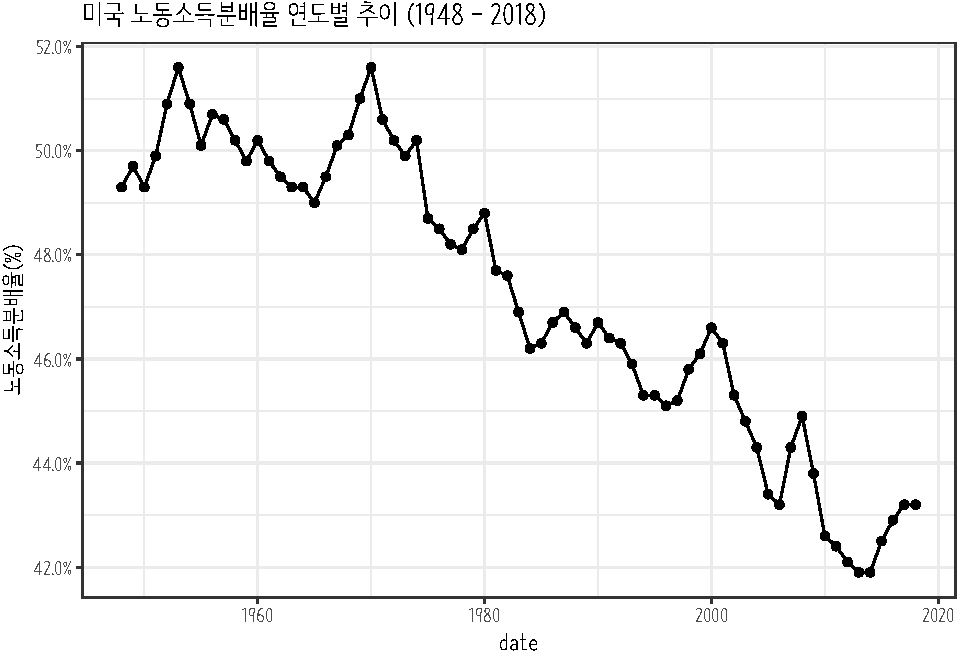
\includegraphics{paper_files/figure-latex/labor-share-us-1} \end{center}

\hypertarget{labor-participation}{%
\subsection{노동인력 참여율}\label{labor-participation}}

\href{https://research.stlouisfed.org/docs/api/api_key.html}{Federal
Reserve Bank of ST. Louis} 웹사이트에서 API-KEY 발급받아
\texttt{usethis::edit\_r\_environ()} 명령어를 통해서 API 키를 잘
관리한다.

\texttt{fredr} 팩키지를 활용하여 직접 웹사이트에서 크롤링하는 번거러움을
해결한다. \texttt{fredr\_set\_key(FRED\_KEY)} 명령어로 API-KEY를
설정한다.

\begin{center}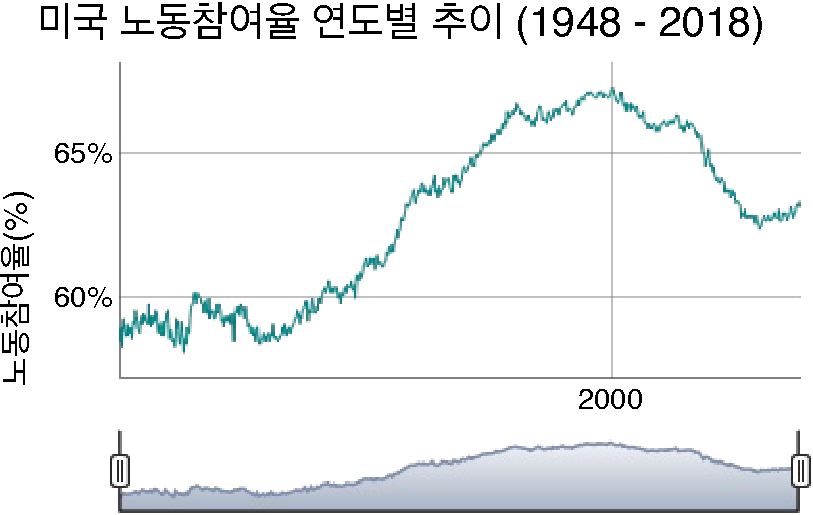
\includegraphics{paper_files/figure-latex/fred-data-labor-participation-1} \end{center}

\hypertarget{automation-overview}{%
\section[자동화]{\texorpdfstring{자동화\footnote{\href{https://hal.pratt.duke.edu/sites/hal.pratt.duke.edu/files/u10/IS-29-05-Expert\%20Opinion\%5B1\%5D_0.pdf}{Mary
  (Missy) Cummings, ``Man versus Machine or Man + Machine?'', Ieee
  INteLLIGeNt sYstems}}}{자동화}}\label{automation-overview}}

기계(Machine)하면 우선 기계장치를 떠올릴 수 있지만, 영어로
머신(machine)은 인공지능을 탑재한 컴퓨터도 의미하기 한다. 자동화 수준을
전혀 컴퓨터, 즉 기계의 도움없이 모든 결정과 행동을 사람이 취하는
수준부터, 인간을 배제하고 기계가 모든 의사결정을 내리고 자율적으로 운전,
판결, 세금계산 등등을 하는 완전한 자동화까지로 수준을 나눌 수 있다.
인간의 어떤 영역은 자동화가 많이 진행되었고, 또 다른 영역은 자동화가
진행되고 있거나, 어떤 영역은 거의 완전한 자동화가 진행된 부분도 있다.

\hypertarget{man-human-comparison}{%
\subsection{사람과 기계 비교}\label{man-human-comparison}}

사람과 기계는 서로 다른 잘하는 영역이 나눠져 있었다. 단어를 세고 가장
많이 사용되는 단어를 찾는 것은 컴퓨터에게는 무척이나 쉬운 작업인 반면,
논문이나 책에서 텍스트를 읽고 이해하는 것은 컴퓨터에게 어렵다. 사람은
지루하고 반복되는 문제를 해결하는데 적합하지 않은 반면에 컴퓨터는
추상적이고 일반화하는 작업에는 적합지 않았다. 이런 사실은 1970년대 미국
카네기 멜론 대학 (CMU) 로봇 공학자 한스 모라벡(Hans Moravec) 교수의
\textbf{모라벡의 역설(Moravec's paradox)}로 잘 알려져 있다.

\begin{table}[H]
\centering
\resizebox{\linewidth}{!}{
\begin{tabular}{lll}
\toprule
속성 & 사람 & 기계\\
\midrule
\rowcolor{gray!6}  속도 & 상대적으로 느림 & 탁월함\\
경격출력 & 상대적으로 약함 & 일관된 작업에 우수성을 보임\\
\rowcolor{gray!6}  일관성 & 믿을 수 없는 학습능력과 피로 & 일관되고 반복적인 작업에 이상적임\\
정보처리능력 & 주로 한개 채널 & 멀티 채널\\
\rowcolor{gray!6}  기억 & 원칙과 전략에 좋음. 다재다능하고 혁신적임 & 문자 그대로 재현하는데 이상적임, 형식적임\\
\addlinespace
추론 계산 & 귀납적, 프로그램하기 더 좋고, 느리고, 오류 수정 좋음 & 연역적, 프로그램하기 귀찮고, 빠르고 정확, 오류 수정 나쁨\\
\rowcolor{gray!6}  감지(sensing) & 넓은 감지 반경, 다기능, 분별력 & 정량적 평가에 좋지만, 패턴인식에는 나쁨\\
인지(perceiving) & 변화에 더 잘 대응 & 잡음에 취약하여 변화에 잘 대응 못함.\\
\bottomrule
\end{tabular}}
\end{table}

\textbf{모라벡의 역설(Moravec's paradox)}

미국 카네기 멜론 대학 (CMU) 로봇 공학자 한스 모라벡(Hans Moravec)이
1970년대에 `it is comparatively easy to make computers exhibit adult
level performance on intelligence tests or playing checkers, and
difficult or impossible to give them the skills of a one-year-old when
it comes to perception and mobility'라는 표현으로 컴퓨터와 인간의 능력
차이를 역설적으로 표현하였다.

즉, 인간은 걷기, 느끼기, 듣기, 보기, 의사소통 등의 일상적인 행위는 매우
쉽게 할 수 있는 반면 복잡한 수식 계산 등을 하기 위해서는 많은 시간과
에너지를 소비하여야 하는 반면, 컴퓨터는 인간이 하는 일상적인 행위를
수행하기 매우 어렵지만 수학적 계산, 논리 분석 등은 순식간에 해낼 수
있다.

\begin{figure}
\centering
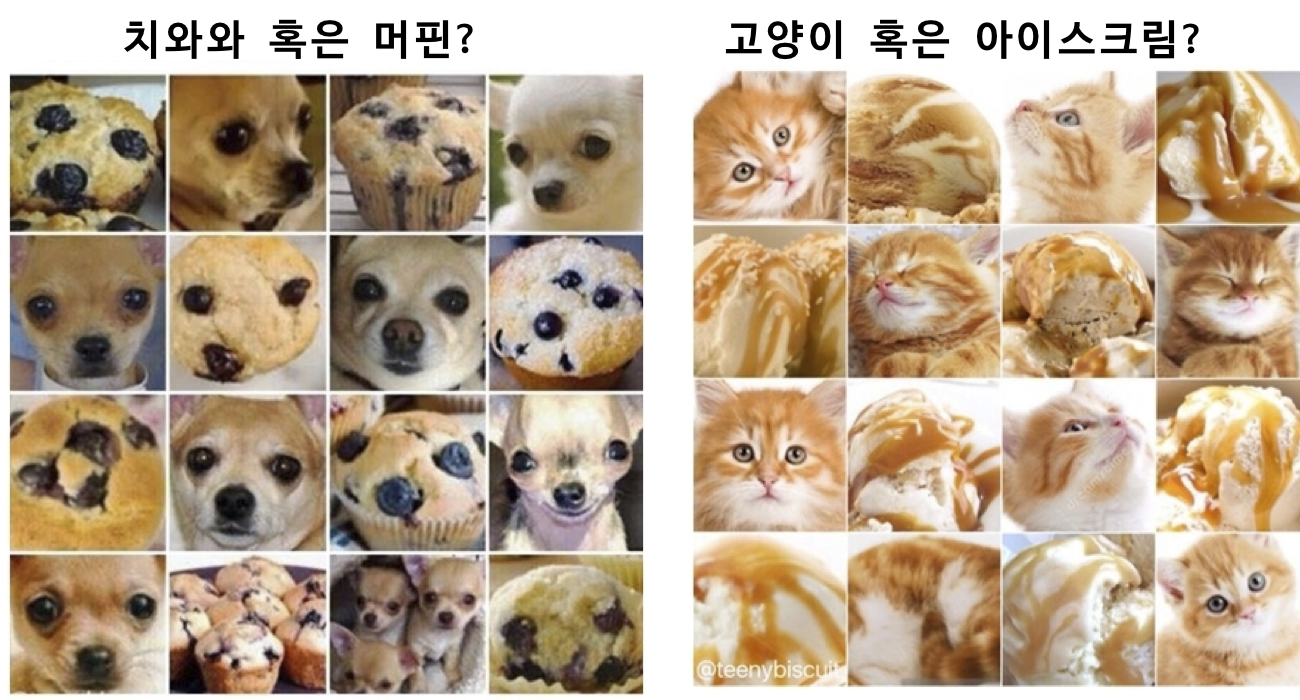
\includegraphics{fig/moravec-paradox.png}
\caption{모라벡의 역설: 치와와와 머핀, 아이스크림과 고양이}
\end{figure}

\hypertarget{chinese-room}{%
\subsection[중국어 방 주장]{\texorpdfstring{중국어 방
주장\footnote{\href{http://ko.experiments.wikidok.net/wp-d/592f718da44f1a4153e80611/View}{중국어
  방 역설 (Chinese room argument) - 대체 누가 중국어를 이해하고 있는가?}}\footnote{\href{https://ko.wikipedia.org/wiki/\%EC\%A4\%91\%EA\%B5\%AD\%EC\%96\%B4_\%EB\%B0\%A9}{위키백과,
  ``중국어 방''}}}{중국어 방 주장}}\label{chinese-room}}

중국어 방 혹은 중국인 방(영어: Chinese room)은 존 설(John Searle)이 튜링
테스트로 기계의 인공지능 여부를 판정할 수 없다는 것을 논증하기 위해
고안한 사고실험이다.

\begin{quote}
우선 방 안에 영어만 할 줄 아는 사람이 들어간다. 그 방에 필담을 할 수
있는 도구와, 미리 만들어 놓은 중국어 질문과 질문에 대한 대답 목록을
준비해 둔다. 이 방 안으로 중국인 심사관이 중국어로 질문을 써서 안으로
넣으면 방 안의 사람은 그것을 준비된 대응표에 따라 답변을 중국어로 써서
밖의 심사관에게 준다.
\end{quote}

안에 어떤 사람이 있는지 모르는 중국인이 보면 안에 있는 사람은 중국어를
할 줄 아는 것처럼 보인다. 그러나, 안에 있는 사람은 실제로는 중국어를
전혀 모르는 사람이고, 중국어 질문을 이해하지 않고 주어진 표에 따라
대답할 뿐이다. 이로부터 중국어로 질문과 답변을 완벽히 한다고 해도 안에
있는 사람이 중국어를 진짜로 이해하는지 어떤지 판정할 수 없다는 결론을
얻는다. 이와 마찬가지로 지능이 있어서 질문 답변을 수행할 수 있는 기계가
있어도 그것이 지능을 가졌는지는 \textbf{튜링 테스트}로는 판정할 수
없다는 주장이다.

\begin{figure}
\hypertarget{id}{%
\centering
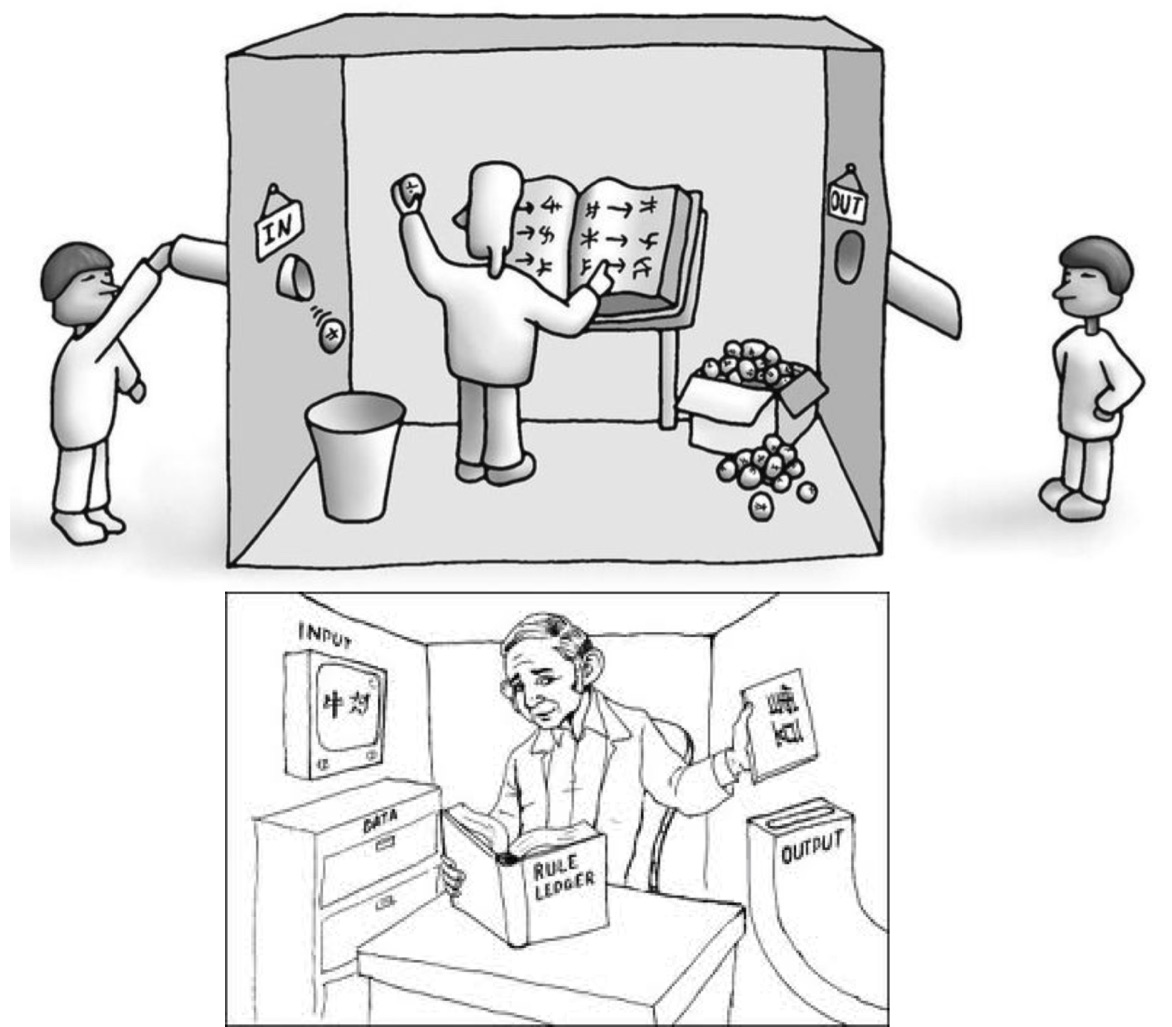
\includegraphics[width=0.77\textwidth,height=\textheight]{fig/chinese-room-argument.jpg}
\caption{중국어 방 주장을 모사한 도해}\label{id}
}
\end{figure}

결국 다음과 같이 컴퓨터, 인간, 인공지능을 비교할 수 있다. 중국어 방이
하드웨어, 인간의 외형적인 몸체라면, 질문과 답변을 입출력으로 정의할 수
있고, 질문\&대답 목록과 처리 규칙을 담은 알고리즘을
데이터베이스/알고리즘, 습득된 경험, 지식, 지능으로 대응할 수 있다.

\begin{table}[H]
\centering
\resizebox{\linewidth}{!}{
\begin{tabular}{l|l|l}
\hline
인공지능 & 컴퓨터 & 인간\\
\hline
\rowcolor{gray!6}  중국어 방 & 하드웨어 & 인간의 외형적인 몸체\\
\hline
영어만 할 줄 아는 사람 & 소프트웨어 & 인간의 지능\\
\hline
\rowcolor{gray!6}  중국어로 된 질문 & 입력(Input) & 인간이 외부에서 접할 수 있는 자극\\
\hline
중국어로 된 답변 & 출력(Output) & 인간이 외부에서 접한 자극에 대한 반응\\
\hline
\rowcolor{gray!6}  질문\&대답 목록 & 데이터베이스(Database) & 습득된 기억\\
\hline
\end{tabular}}
\end{table}

\hypertarget{man-human-boundary}{%
\section{사람과 기계 업무 분장}\label{man-human-boundary}}

앞서 자동화 수준을 1-10 사이로 구분했다면, 사람과 기계 사이의 업무 분장
경계를 적당히 지어야만 해당 문제를 자동화를 통해서 최선의 결과를 낼 수
있다. 오랜동안 논란이 되었지만, 대표적으로 달에 사람을 보내는 아폴로
계획에서 사람과 기계의 역할을 어떻게 구분하는 것이 좋은지는 항상 논란이
되어왔고 오늘날까지 이어지고 있다.

\begin{figure}
\hypertarget{id}{%
\centering
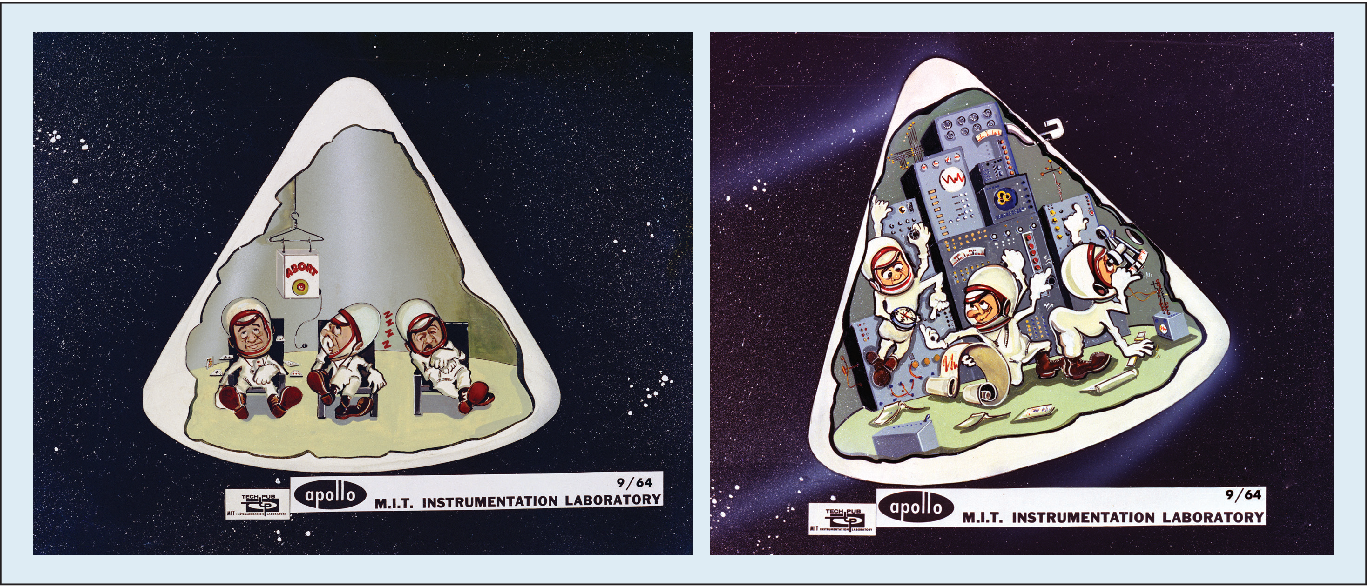
\includegraphics[width=1\textwidth,height=\textheight]{fig/man-machine-role-allocation.png}
\caption{아폴로 계획에 대한 역할 구분}\label{id}
}
\end{figure}

듀크 대학과 MIT 매리 커밍스(Mary Cummings) 교수는 기존 S-R-K 틀에 E를 더
붙이는 등 확장을 하여 다음과 같은 기계와 사람이 잘하는 분야, 즉 자동화가
되는 영역과 자동화의 도움을 받는 영역으로 범주화 시켰다. 매리 커밍스
교수가 F-18 여성 조종사 경력을 바탕으로 항공 사례를 예시로 들고 있다.

\textbf{인지작업과 자동화 정도}

\textbf{Skill-Rule-Knowledge-Experties}

최근 자동화 기계는 드론, 무인 자동차, 무인 화물자동차, 무인 비행기, 무인
선박 모두 센서와 액추에이터를 통해서 자동으로 설정한 목표를 달성하게
되어 있지만 이는 중앙 컴퓨터의 제어를 받는다. 중앙 컴퓨터 제어는 결국
사람이 화면을 보고 제어 로직을 심어둔 것으로 크게 볼 수 있다.

\begin{figure}
\hypertarget{id}{%
\centering
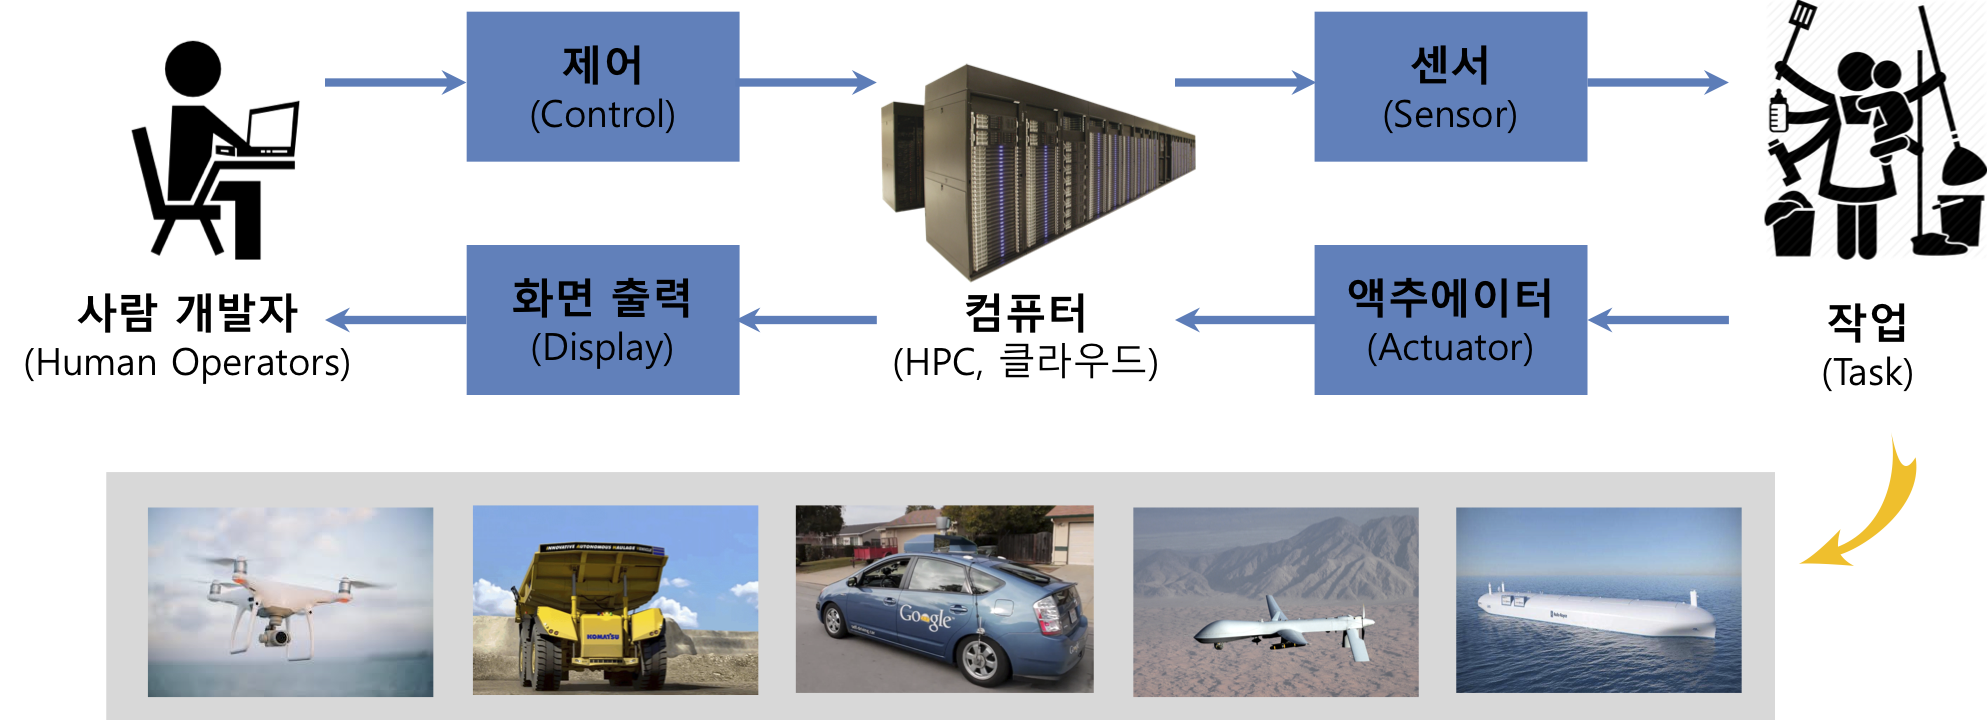
\includegraphics[width=1\textwidth,height=\textheight]{fig/human-supervisory-control.png}
\caption{human-supervisory-control}\label{id}
}
\end{figure}

\hypertarget{play-go}{%
\subsection[이세돌 9단]{\texorpdfstring{이세돌
9단\footnote{\href{https://n.news.naver.com/article/092/0002175655}{이균성(2019.11.28),
  ``이세돌 9단의 프로기사 포기는 `노동의 미래'다'', ZDNET Korea}}}{이세돌 9단}}\label{play-go}}

이창호를 누르고 바둑 최강자에 굴림해온 전설적인 이세돌 9단. 하지만
알파고가 나온 이후 모든 것이 바뀌었다. 커제는 알파고와 대결에서 울기도
했고, 5명의 프로기사가 때로 알파고에 덥비기도 했다. 그렇다고 결과가 바뀐
것은 아니다. NHN에서 20년동안 학습한 바둑 프로그램 한돌과 2점 깔고 두는
접바둑으로 마지막 대국을 남기고 평생을 함께 한 바둑을 놓으려고 한다.

\hypertarget{challenge-to-human}{%
\section[기계에 대체되는 일자리]{\texorpdfstring{기계에 대체되는
일자리\footnote{\href{https://medium.com/@jonathan_hui/gan-some-cool-applications-of-gans-4c9ecca35900}{Jonathan
  Hui (2018), ``GAN -Some cool applications of GANs.''}}\footnote{\href{https://machinelearningmastery.com/impressive-applications-of-generative-adversarial-networks/}{Jason
  Brownlee (June 14, 2019), ``18 Impressive Applications of Generative
  Adversarial Networks (GANs)''}}}{기계에 대체되는 일자리}}\label{challenge-to-human}}

사람이 가지고 있는 오감(시각, 후각, 청각, 촉각, 미각) 중에서 시각을
대부분의 사람들은 가장 중요한 감각이라고 꼽는데 이유는 아마도 감각기관을
통해서 획득하는 정보의 90\% 이상이 시각을 통해서 얻어진다는 점에
기인한다.

\begin{figure}
\hypertarget{id}{%
\centering
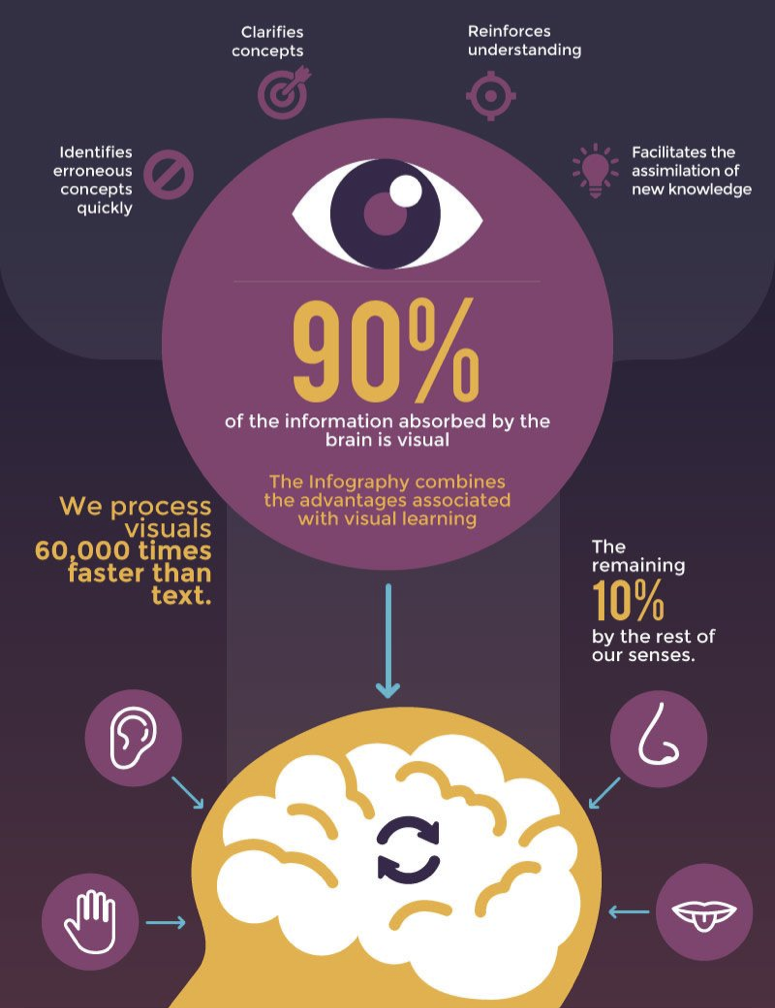
\includegraphics[width=0.5\textwidth,height=\textheight]{fig/sensory-visual.png}
\caption{시각의 중요성 - 정보 처리 90\%이상}\label{id}
}
\end{figure}

\textbf{GAN(Generative Adversarial Network)}은 생성적 적대 신경망라고
번역할 수 있다. 이안 굿펠로우(Ian Goodfellow)가 NIPS 학회에서 발표한
뒤로 딥러닝의 대가인 얀 르쿤(Yann Lecun) 교수는 GAN을 최근 10년간
머신러닝 연구 중 가장 혁신적인 아이디어로 극찬했다.

\textbf{생성 모델링 과정}

\begin{figure}
\centering
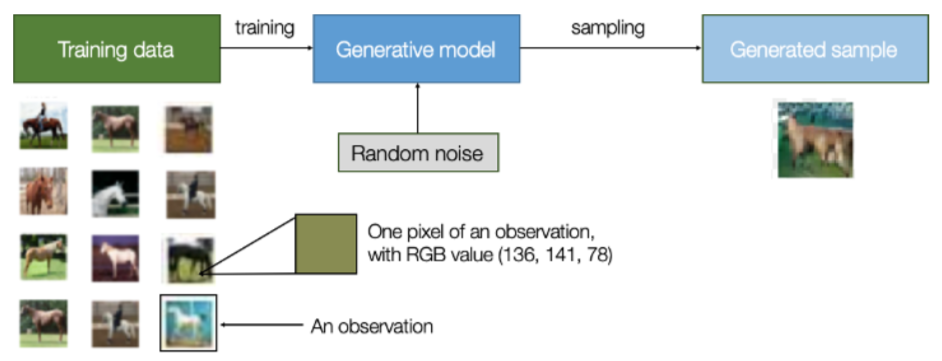
\includegraphics{fig/generative-model.png}
\caption{생성 모델링 과정}
\end{figure}

\textbf{판별 모델링 과정}

\begin{figure}
\centering
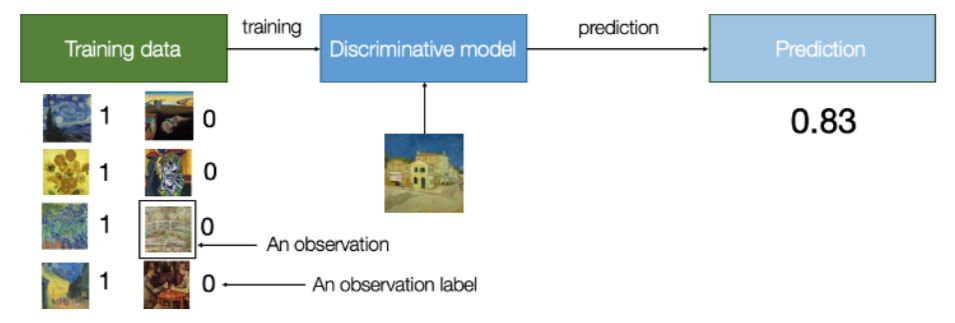
\includegraphics{fig/discriminative-model.png}
\caption{판별 모델링 과정}
\end{figure}

\hypertarget{challenge-to-human-paint}{%
\subsection{페인트(paint)}\label{challenge-to-human-paint}}

\href{https://github.com/eriklindernoren/Keras-GAN}{Keras-GAN} GitHub
사이트에는 \texttt{pix2pix}, \texttt{CycleGAN}을 포함한 다양한 시각적인
사례를 살펴볼 수 있다.

\begin{itemize}
\tightlist
\item
  이미지 생성(Image generation): GAN을 사용하여 이미지를 기계가 자동으로
  생성할 수 있다. 예를 들어 자동 로고생성기 등.
  \href{https://github.com/alex-sage/logo-gen}{GitHub:
  alex-sage/logo-gen}
\item
  텍스트로 이미지 합성 (Text-to-image synthesis): 영화산업에서
  시나리오가 있는 상태에서 텍스트를 기초로 하여 이미지를 자동 생성시킴.
  \href{https://medium.com/datadriveninvestor/text-to-image-synthesis-6e5de1bf86ec}{Nikunj
  Gupta, ``Text-to-Image Synthesis'', Medium},
  \href{https://github.com/crisbodnar/text-to-image}{GitHub,
  text-to-image}
\item
  얼굴 노화(Face Aging): 연애 산업과 보안산업에서 특히 유용한데 보안의
  경우 얼굴 노화과정을 GAN을 통해 모델을 갖춤으로써 직원의 노화에 따라
  신규 시스템으로 바꿀 필요가 없다.
  \href{https://github.com/yuanzhaoYZ/Face-Aging-CAAE}{GitHub,
  yuanzhaoYZ/Face-Aging-CAAE}
\item
  이미지를 다른 이미지로 번역(image-to-image-translation): 흑백이미지를
  칼러 이미지로, 스케치 이미지를 색칠된 이미지로, 이미지를 피카소나
  반고흐 스타일로 번역하는 것을 통해 시간을 상당히 줄일 수 있다.
  \href{https://github.com/topics/image-to-image-translation}{GitHub
  topics: image-to-image-translation}
\item
  고화질 이미지 생성(High-resolution image generation): 저해상도 카메라
  이미지를 고화질 이미지로 변환.
  \href{https://github.com/david-gpu/srez}{david-gpu/srez}
\item
  결측된 이미지 채워넣기(completing missing parts of images): 이미지의
  빠진 부분을 채워넣거나 불필요한 부분이 있다면 지워서 결측시킨 후에
  이미지를 채워넣는다.
  \href{https://github.com/topics/image-completion}{Github topic:
  image-completion}
\end{itemize}

\hypertarget{writing-machine}{%
\subsection{자작(write)}\label{writing-machine}}

\begin{itemize}
\tightlist
\item
  \href{https://github.com/topics/text-generation}{GitHub topic:
  text-generation}

  \begin{itemize}
  \tightlist
  \item
    \href{https://github.com/Maluuba/newsqa}{Maluuba NewsQA dataset}
  \item
    \href{https://github.com/Maluuba/qgen-workshop}{Multi-task Question
    and Answer Generation}
  \end{itemize}
\end{itemize}

\hypertarget{music-machine}{%
\subsection{음악(music)}\label{music-machine}}

\begin{itemize}
\tightlist
\item
  \href{https://salu133445.github.io/musegan/}{museGAN}
\item
  \href{https://medium.com/@rachelchen_49210/generating-ambient-noise-from-wavenet-95aa7f0a8f77}{Rachel
  Chen (Dec 13, 2017), ``Generating Ambient Music from WaveNet'',
  Medium}
\item
  \href{https://github.com/tensorflow/magenta}{tensorflow/magenta}
\item
  \href{https://towardsdatascience.com/generating-pokemon-inspired-music-from-neural-networks-bc240014132}{Abraham
  Khan(Dec 15, 2018), ``Generating Pokemon-Inspired Music from Neural
  Networks'', Medium}
\end{itemize}

\hypertarget{play-machine}{%
\subsection{연극(play)}\label{play-machine}}

\begin{itemize}
\tightlist
\item
  \href{https://worldmodels.github.io/}{World Models}
\item
  \href{https://dylandjian.github.io/world-models/}{Dylan's blog (June
  06, 2018), ``World Models applied to Sonic''}
\end{itemize}

한글(참고 Brynjolfsson and McAfee
\protect\hyperlink{ref-brynjolfsson2014second}{2014}\}).
\cite{Galyardt14mmm}. \ref{sec:1}

한글 is best by\textasciitilde{}\cite{brynjolfsson2014second}

\hypertarget{refs}{}
\begin{cslreferences}
\leavevmode\hypertarget{ref-brynjolfsson2014second}{}%
Brynjolfsson, Erik, and Andrew McAfee. 2014. \emph{The Second Machine
Age: Work, Progress, and Prosperity in a Time of Brilliant
Technologies}. WW Norton \& Company.
\end{cslreferences}

\bibliographystyle{spbasic}
\bibliography{bibliography.bib}

\end{document}
